\documentclass{article}
\usepackage{amsthm}
\usepackage{graphicx}
\usepackage{subfig}
\usepackage{physics}
\graphicspath{ {figures/} }

\title{The Tight Binding Model}
\author{Caitlin Carnahan}
\begin{document}
\maketitle
\begin{abstract}
This document is intended as a detailed review of covalent bonding and the Tight Binding (LCAO) model in preparation for study of monolayer and bilayer graphene.
\end{abstract}
\section{Covalent Bonding}
Graphene is composed of hexagonally-shaped links of carbon atoms, each of which is linked to three other carbon atoms when the hexagons are tiled. These carbon atoms are linked together by covalent bonds.
The purpose of this section is to review the fundamental concepts of covalent bonding, as well as the properties of the carbon atom itself. \par
Carbon is the chemical element with atomic number 6 - that is, there are six protons found in the nucleus of a Carbon atom. The ground-state electron configuration of Carbon is $1s^{2}2s^{2}2p^{2}$. However, when in the presence of other atoms,
it is sometimes energetically favorable to promote one electron into the $2p$ orbital - the energy cost of moving into this excited state is offset by the energy gained from covalent bonding. \par
In the case of graphene, carbon atoms exibit $sp^{2}$ hybridization wherein two $2p$ orbitals, conventionally chosen as $2p_{x}$ and $2p_{y}$, form a superposition with the $2s$ orbital. The result is three coplanar orbitals separated by $120^{\circ}$.
The remaining $2p_{z}$ orbital lies perpendicular to the coplanar hybridized orbitals. Sheets of graphene are formed by planes of carbon atoms bonding via the hybridized orbitals, but this leaves the perpendicular $2p_{z}$ orbital free. \par
We now turn our attention to the nature of covalent bonding in graphene. What follows is a description of covalent bonding that closely follows that presented in \cite{oxford}. As a simple model, we can demonstrate the energetically favorable effects
produced by covalent bonding if we imagine an atom as a potential well for an electron - specifically, we model an atom as an infinite square well.
\begin{figure}[h]
\centering
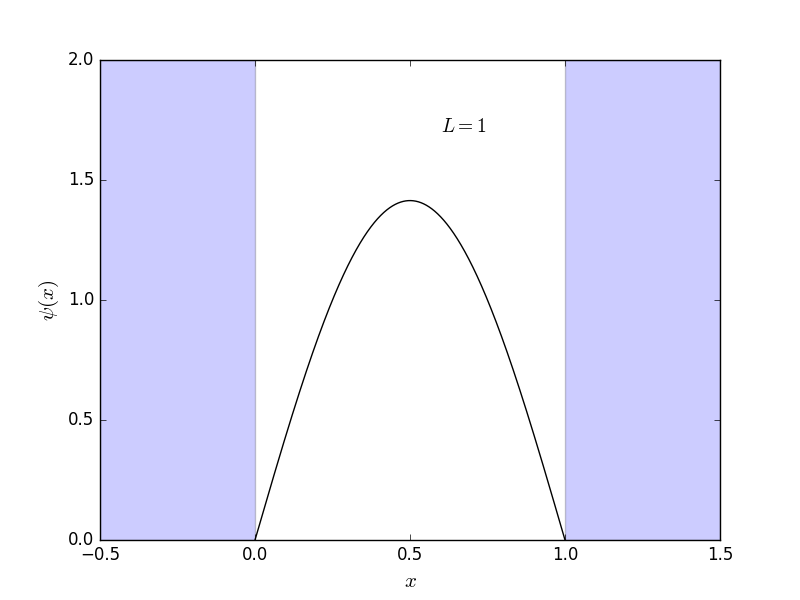
\includegraphics[scale=.5]{figure_1}
\caption{The ground state $\psi(x)$ for the case $L = 1$.}
\end{figure}
The ground state energy for a single electron in the infinite square well is given by: $$E = \frac{\pi^{2}\hbar^{2}}{2mL^{2}}$$
and the ground state solution is $$\psi(x) = \sqrt{\frac{2}{L}}sin\left (\frac{\pi x}{L}\right )$$ If we have two such atoms and we bring them close enough together, a single electron can be found in the shared space produced by doubling the well width. If the well width is doubled
to $2L$, then the ground state energy becomes $$E = \frac{\pi^{2}\hbar^{2}}{2m(2L)^{2}}$$ Therefore, doubling the well width decreases the ground state energy by a factor of 4.
\begin{figure}[h]
\centering
\subfloat{{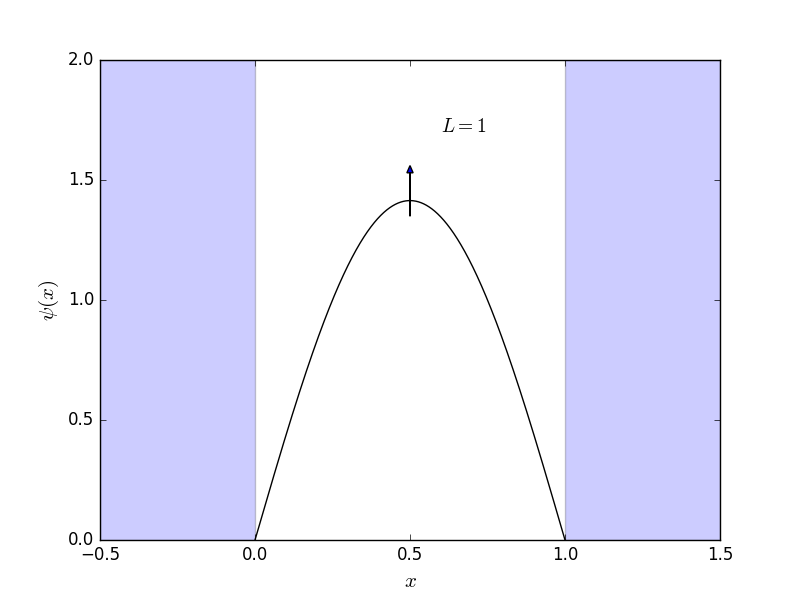
\includegraphics[scale=.28]{figure_2_up}}}%
\qquad
\subfloat{{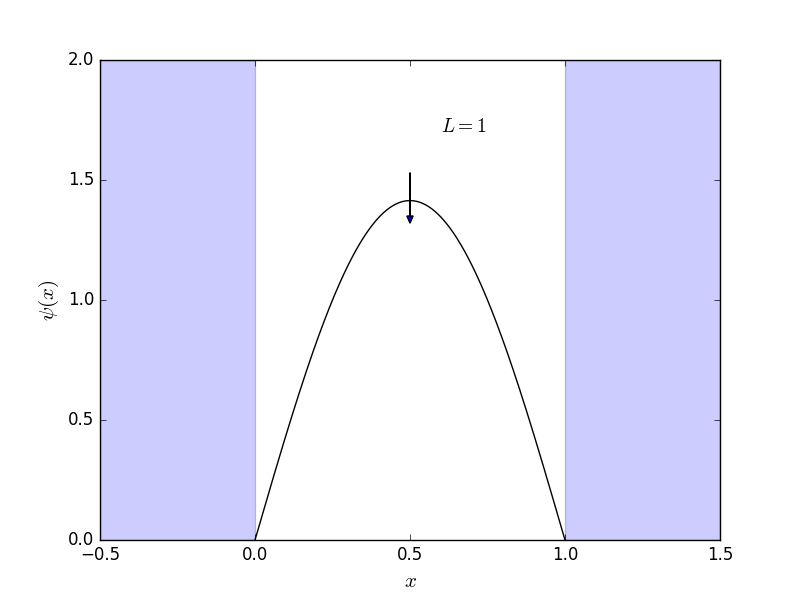
\includegraphics[scale=.28]{figure_2_down}}}%
\caption{The individual ground state $\psi(x)$ for the case $L = 1$ shown for each atom - one with elecron spin up and the other with spin down.}
\end{figure}

This simple model demonstrates the motivation for covalent bonding: delocalizing the electron is energetically favorable
because the new ground state (the \emph{bonding} orbital) is lower in energy than the original ground state. This principle holds even when considering one electron on each of the two atoms -- both electrons can occupy the new lower-energy bonding orbital if they have opposite spin states. However, covalent bonding is not energetically favorable in every situation - \emph{antibonding} orbitals can be produced that offset the decrease in energy due to the bonding orbital.

\begin{figure}[h]
\centering
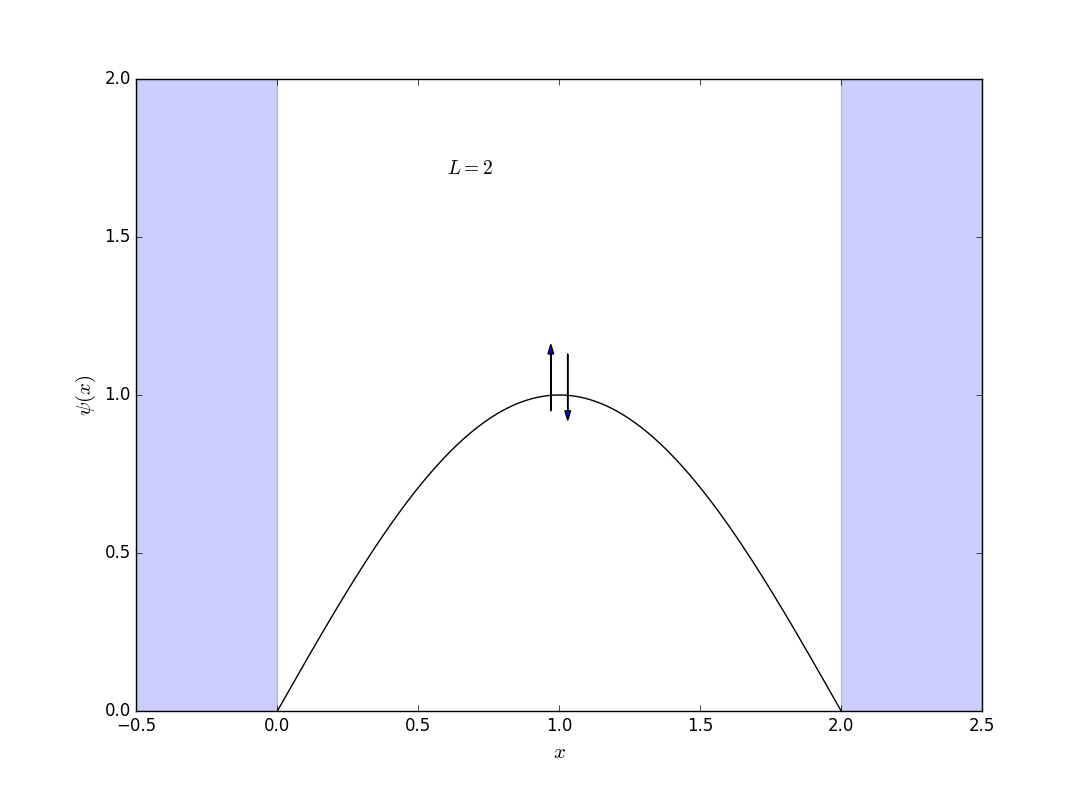
\includegraphics[scale=.4]{figure_2_both}
\caption{The new ground state $\psi(x)$ for the case $L = 2$ with two spin states.}
\end{figure}

\section{Tight Binding Model}
\subsection{Introduction: Two Hydrogen Atoms}
We begin our discussion of the tight binding model by considering a simple system of two hydrogen atoms. Each hydrogen atom has a single electron orbiting its nucleus. Individually,
the ground state of an electron orbiting a hydrogen nucleus has the form
$$ \psi(r) = \frac{1}{\sqrt{\pi}a_{0}^{3/2}}e^{-r/a_{0}}$$
and exhibits the following radial probability density, plotted in Figure 4 with $a_{0} = 1$.
$$ P(r) = \int_{V} \left | \psi(r)\right |^{2} rsin(\theta)drd\theta d\phi= \left ( \frac{4r^{2}}{a_{0}^3}\right )e^{-2r/a_{0}}$$
In the region $0 \geq r \leq 2a_{0}$, this probability distribution is roughly equivalent to the infinite square well probability distribution, also shown in Figure 4. So, we can
clearly model the hydrogen atom as a square potential well.
\begin{figure}[h]
\centering
\subfloat{{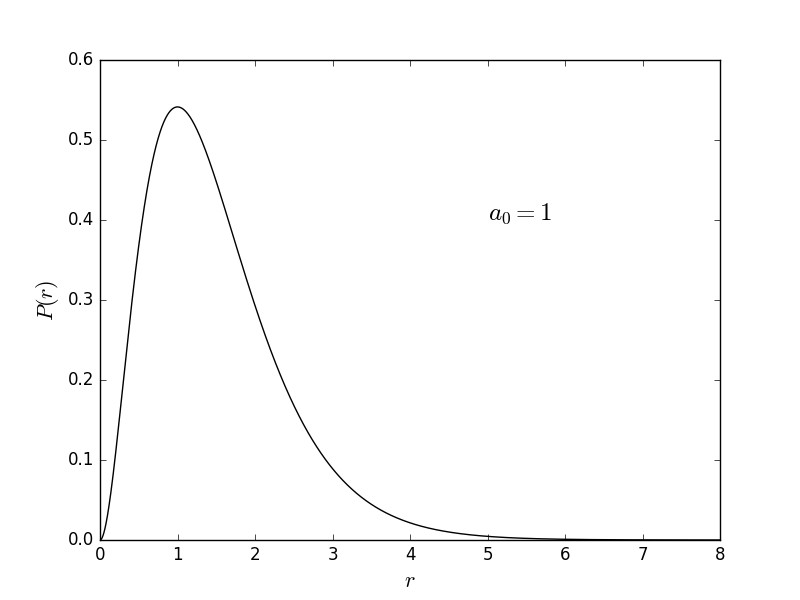
\includegraphics[scale=.28]{figure_4}}}%
\qquad
\subfloat{{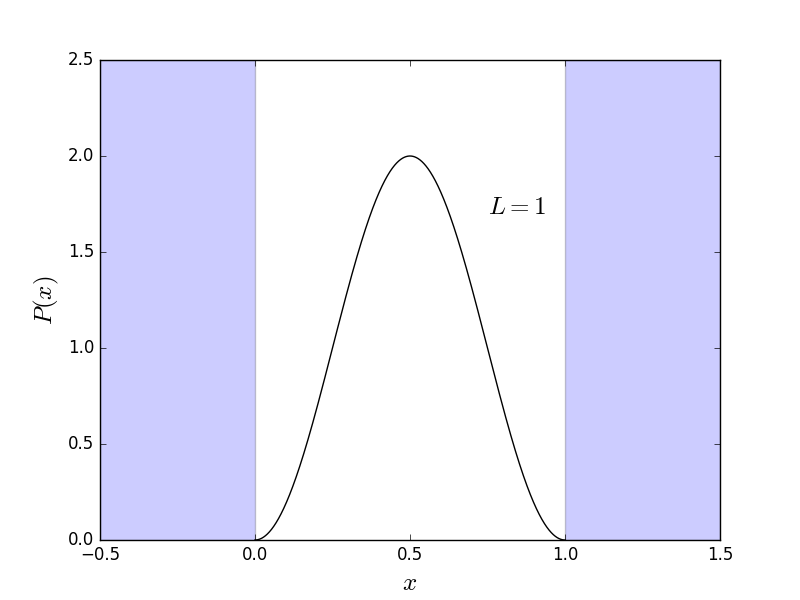
\includegraphics[scale=.28]{figure_4_isw}}}%
\caption{The radial probability distribution for the ground state of hydrogen. The radius of highest probability corresponds to the bohr radius $a_{0}$, which is set to 1 here. Also
shown is the positional probability distribution of the infinite square well of length $L = 1$.}
\end{figure}

Now, when we bring the two hydrogen atoms close to one another, the well width doubles and the individual wave functions overlap as shown in Figure 5 (TO DO: finish potential well explanation.). \par

Our goal now is to establish a description of the covalently bonded system through the use of a linear combination of ground state orbitals. Let $\ket{\psi_{0,1}}$ and $\ket{\psi_{0,2}}$
be the ground states of the first and second hydrogen atom, respectively. Then, $\ket{\psi_{0,1}}$ and $\ket{\psi_{0,2}}$ are clearly solutions to the Schroedinger equations
$$H\ket{\psi_{0,1}} = (K + V_{1})\ket{\psi_{0,1}} = E_{0}\ket{\psi_{0,1}} $$
$$H\ket{\psi_{0,2}} = (K + V_{2})\ket{\psi_{0,2}} = E_{0}\ket{\psi_{0,2}}$$
where $K$ is the kinetic energy of the electron, and $V_{i}$ is the nuclear potential from site $i$. We will describe the ground state of a single electron orbiting the two hydrogen neighbors as a linear combination of these individual ground states. That is,
$$ \ket{\psi_{0}} = c_{1}\ket{\psi_{0,1}} + c_{2}\ket{\psi_{0,1}}  $$
We can roughly approximate $\ket{\psi_{0,1}}$ and $\ket{\psi_{0,2}}$ to be orthogonal. As shown in Figure 5 (TO BE ADDED), the individual ground states are localized to either side of the potential well and
there is little overlap between the states given that the internucleic distance is not too short. This approximation allows us to establish the following orthogonality condition.
$$ \bra{\psi_{0,i}}\ket{\psi_{0,j}} = \delta_{ij}$$.
Now we will attempt to solve the Schroedinger equation to find the new ground state energy of the bonded system. The Schroedinger Equation is simply
$$H\ket{\psi_{0}} = E\ket{\psi_{0}}$$
We have not yet established the form of the Hamiltonian, but we can make two observations. The first is that the Hamiltonian can be written as the sum of the kinetic energy of the electron, as well as the potential energy contributions from each
of the hydreogen nuclei. That is,
$$ H = K + V_{1} + V_{2}$$
The second observation is that the Schroedinger equation can be written in a more explicit form. In this case, the new bonding ground state is a linear combination of two ground state orbitals - therefore, the
Hamiltonian is a $2\times 2$ matrix.
$$ \begin{bmatrix} H_{11} & H_{12}\\ H_{21}&H_{22} \end{bmatrix}\begin{bmatrix} c_{1} \\ c_{2} \end{bmatrix} = E\begin{bmatrix} c_{1} \\ c_{2} \end{bmatrix}$$
This yields the following system of equations
$$\sum_{j}H_{ij}c_{j} = Ea_{i}$$
where
$$H_{ij} = \bra{\psi_{0,i}}H\ket{\psi_{0,j}} = \bra{\psi_{0,i}}K + V_{1} + V_{2}\ket{\psi_{0,j}}$$
This allows us to examine the components of the Hamiltonian matrix.
$$H_{11} = \bra{\psi_{0,1}}K + V_{1}\ket{\psi_{0,1}} + \bra{\psi_{0,1}}V_{2}\ket{\psi_{0,1}} = E_{0} + V_{cross}$$
$$H_{22} = \bra{\psi_{0,2}}K + V_{2}\ket{\psi_{0,2}} + \bra{\psi_{0,2}}V_{1}\ket{\psi_{0,2}} = E_{0} + V_{cross}$$
$$H_{12} = \bra{\psi_{0,1}}K + V_{2}\ket{\psi_{0,2}} + \bra{\psi_{0,1}}V_{1}\ket{\psi_{0,2}} = -t$$
$$H_{21} = \bra{\psi_{0,2}}K + V_{2}\ket{\psi_{0,1}} + \bra{\psi_{0,2}}V_{1}\ket{\psi_{0,1}} = -t^{*}$$
where we have defined $V_{cross} = \bra{\psi_{0,2}}V_{1}\ket{\psi_{0,2}} = \bra{\psi_{0,1}}V_{2}\ket{\psi_{0,1}}$ and the \emph{hopping} term $ -t = \bra{\psi_{0,1}}V_{1}\ket{\psi_{0,2}}$. The $V_{cross}$ term represents the Coulomb potential
due to neighboring sites (i.e. the \emph{other} hydrogen nucleus). The hopping element $t$ represents the mechanism by which the electron can move from one orbital to another. To obtain the eigenenergies, we can diagonalize this Hamiltonian as follows.
$$det(H - EI) = \begin{vmatrix} E_{0} + V_{cross} - E & -t \\ -t^{*} & E_{0} + V_{cross} - E\end{vmatrix} = 0$$
From which we obtain
$$  (E_{0} + V_{cross} - E)^{2} - |t|^{2} = 0$$
$$ E^{2} - 2E(E_{0} + V_{cross}) + (E_{0} + V_{cross})^{2} - |t|^{2} = 0$$
Using the quadratic equation, we obtain the solution
$$E_{\pm} = E_{0} + V_{cross} \pm |t|$$
Now, we will find the eigenstates associated with the new ground state energies. The Schroedinger equation, again, is
$$ \begin{bmatrix} E_{0} + V_{cross} & -t\\ -t^{*} & E_{0} + V_{cross} \end{bmatrix}\begin{bmatrix} c_{1} \\ c_{2} \end{bmatrix} = E_{\pm}\begin{bmatrix} a_{1} \\ a_{2} \end{bmatrix}$$
which gives us the following system of equations to solve for $c_{1}$ and $c_{2}$
$$ (E_{0} + V_{cross})c_{1} -tc_{2} = E_{\pm}c_{1} $$
$$ (E_{0} + V_{cross})c_{2} -t*c_{1} = E_{\pm}c_{2} $$
Our associated normalized eigenvectors are therefore
$$\ket{\psi_{+}} = \frac{1}{\sqrt{2}}\ket{\psi_{0,1}} - \frac{1}{\sqrt{2}}\ket{\psi_{0,2}}$$
$$\ket{\psi_{-}} = \frac{1}{\sqrt{2}}\ket{\psi_{0,1}} + \frac{1}{\sqrt{2}}\ket{\psi_{0,2}}$$
The first thing to notice here is that while the individual hydrogen atoms have a single ground state orbital, when the atoms are brought close together, the delocalized ground state orbital actually splits into two levels.
The lower energy level (with energy $E_{-}$) is called the \emph{bonding} orbital because it promotes bonding by lowering the ground state energy. The higher energy orbital (associated with $E_{+}$) is called the \emph{antibonding} orbital. This is somewhat easier to understand
if we factor in Coulomb repulsion between the neighboring nuclei and allow the $V_{cross}$ term to vanish. In that case, we have
$$ E_{\pm} = E_{0} \pm |t| $$
So clearly, the bonding orbital has an energy lower than the original ground state energy and the antibonding orbital is associated with an energy higher than the original ground state energy. It is also worth noting that the difference between the bonding and antibonding energy levels is
proportional to the hopping term. In the limit that the hopping term vanishes, indicating that there is no possibility to hop between sites, the ground state energies converge back to the original ground state energy of hydrogen.

\subsection{Next Steps: One Dimensional Chain of Atomic Sites}
We will now generalize our model a bit by considering a one-dimensional chaing of $N$ sites, as opposed to two. First, we establish some properties of
our chain:
\begin{itemize}
\item There is a single orbital on each atomic site -  we will denote the orbital on site $i$ as $\ket{i}$.
\item Periodic boundary conditions are enforced. That is, site $N+1$ is site $1$.
\item Orbitals are taken to be orthogonal to one another. Therefore, $\bra{i}\ket{j} = \delta_{ij}$.
\item The interatomic spacing - distance between sites - is denoted $a$.
\end{itemize}

\begin{thebibliography}{9}
\bibitem{oxford}
Steven H. Simon.
\textit{Lecture Notes for Solid State Physics}.
Oxford University, 2012.

\end{thebibliography}



\end{document}
